% THIS IS SIGPROC-SP.TEX - VERSION 3.1
% WORKS WITH V3.2SP OF ACM_PROC_ARTICLE-SP.CLS
% APRIL 2009
%
% It is an example file showing how to use the 'acm_proc_article-sp.cls' V3.2SP
% LaTeX2e document class file for Conference Proceedings submissions.
% ----------------------------------------------------------------------------------------------------------------
% This .tex file (and associated .cls V3.2SP) *DOES NOT* produce:
%       1) The Permission Statement
%       2) The Conference (location) Info information
%       3) The Copyright Line with ACM data
%       4) Page numbering
% ---------------------------------------------------------------------------------------------------------------
% It is an example which *does* use the .bib file (from which the .bbl file
% is produced).
% REMEMBER HOWEVER: After having produced the .bbl file,
% and prior to final submission,
% you need to 'insert'  your .bbl file into your source .tex file so as to provide
% ONE 'self-contained' source file.
%
% Questions regarding SIGS should be sent to
% Adrienne Griscti ---> griscti@acm.org
%
% Questions/suggestions regarding the guidelines, .tex and .cls files, etc. to
% Gerald Murray ---> murray@hq.acm.org
%
% For tracking purposes - this is V3.1SP - APRIL 2009

\documentclass{sig-alternate-ipsn13}

\newcommand{\hd}{\emph{H+D}}
\newcommand{\hp}{\emph{Hpin}}
\newcommand{\dm}{\emph{Dmap}}
\newcommand{\dmh}{\emph{DmapH}}

%-----------------------------------------
% need for camera-ready
\pagestyle{empty}

%----------------------------------------

\begin{document}

\title{
%Zero-Copy I/O Processing for Low-Latency GPU Computing
Zero-Copy I/O for Low-Latency GPU Computing
}
%
% You need the command \numberofauthors to handle the 'placement
% and alignment' of the authors beneath the title.
%
% For aesthetic reasons, we recommend 'three authors at a time'
% i.e. three 'name/affiliation blocks' be placed beneath the title.
%
% NOTE: You are NOT restricted in how many 'rows' of
% "name/affiliations" may appear. We just ask that you restrict
% the number of 'columns' to three.
%
% Because of the available 'opening page real-estate'
% we ask you to refrain from putting more than six authors
% (two rows with three columns) beneath the article title.
% More than six makes the first-page appear very cluttered indeed.
%
% Use the \alignauthor commands to handle the names
% and affiliations for an 'aesthetic maximum' of six authors.
% Add names, affiliations, addresses for
% the seventh etc. author(s) as the argument for the
% \additionalauthors command.
% These 'additional authors' will be output/set for you
% without further effort on your part as the last section in
% the body of your article BEFORE References or any Appendices.

\numberofauthors{2} %  in this sample file, there are a *total*
% of EIGHT authors. SIX appear on the 'first-page' (for formatting
% reasons) and the remaining two appear in the \additionalauthors section.
%
\author{
% You can go ahead and credit any number of authors here,
% e.g. one 'row of three' or two rows (consisting of one row of three
% and a second row of one, two or three).
%
% The command \alignauthor (no curly braces needed) should
% precede each author name, affiliation/snail-mail address and
% e-mail address. Additionally, tag each line of
% affiliation/address with \affaddr, and tag the
% e-mail address with \email.
%
\alignauthor Shinpei Kato\\
       \affaddr{Dept. Information Engineering}\\
       \affaddr{Nagoya University}
\and
\alignauthor Nikolaus Rath\\
       \affaddr{Dept. Applied Physics and Applied Mathematics}\\
       \affaddr{Columbia University}
\and
\alignauthor Jason Aumiller and Scott Brandt\\
       \affaddr{Dept. Computer Science}\\
       \affaddr{University of California, Santa Cruz}
}
% There's nothing stopping you putting the seventh, eighth, etc.
% author on the opening page (as the 'third row') but we ask,
% for aesthetic reasons that you place these 'additional authors'
% in the \additional authors block, viz.
%\additionalauthors{Additional authors: John Smith (The Th{\o}rv{\"a}ld Group,
%email: {\texttt{jsmith@affiliation.org}}) and Julius P.~Kumquat
%(The Kumquat Consortium, email: {\texttt{jpkumquat@consortium.net}}).}
%\date{30 July 1999}
% Just remember to make sure that the TOTAL number of authors
% is the number that will appear on the first page PLUS the
% number that will appear in the \additionalauthors section.

\maketitle

%-----------------------------------------
% need for camera-ready
\thispagestyle{empty}

\begin{abstract}
 Cyber-physical systems (CPS) often control complex physical
 phenomenon. 
 The computational workload of control algorithms, hence, is becoming a
 core challenge of CPS due to their real-time constraints.
 By nature, control algorithms of CPS exhibit a high degree of data
 parallelism, which can be offloaded to parallel compute devices,
 such as graphics processing units (GPUs).
 Yet another problem is introduced by the communication between the host
 processor and the compute device.
 As a matter of fact, plasma control requires an order of a few
 microseconds for the sampling period, while today's systems may take
 several ten microseconds to copy data between the host and the device
 memory at scale of the required data size.
 In this paper, we present a zero-copy I/O processing scheme that
 enables sensor and actuator devices to directly transfer data to and
 from compute devices without using the host processor.
 The basic idea behind this scheme is to map the I/O address space onto
 the device memory, removing data-copy operations upon the host memory.
 The experimental results from the real-world plasma control
 system demonstrate that a sampling period of plasma control can be
 reduced by 33\% under the zero-copy I/O scheme.
 The microbenchmarking results also show that GPU-accelerated matrix
 computations can be completed in 34\% less time than current methods,
 while effective data throughput is at least as good as the current best
 performers.
\end{abstract}

\keywords{GPGPU, Zero-Copy I/O, Plasma Fusion}

\section{Introduction}
\label{sec:introduction}

Cyber-physical systems (CPS) are next generations of networked and
embedded systems, tightly coupled with computation and physical
elements to control real-world phenomenon.
Control algorithms of CPS, therefore, are becoming more and more
complex, which makes CPS distinguished from traditional safety-critical
systems.
In CPS applications, ``real-fast'' is often as important as ``real-time'',
while safety-critical systems are likely to have only the real-time
constraint. 
Such a double-edge real-time and real-fast requirement of CPS, however,
has imposed a core challenge on systems technology.
In this paper, we tackle this problem with a specific example of plasma
control.

\begin{figure}[tb]
 \centering
 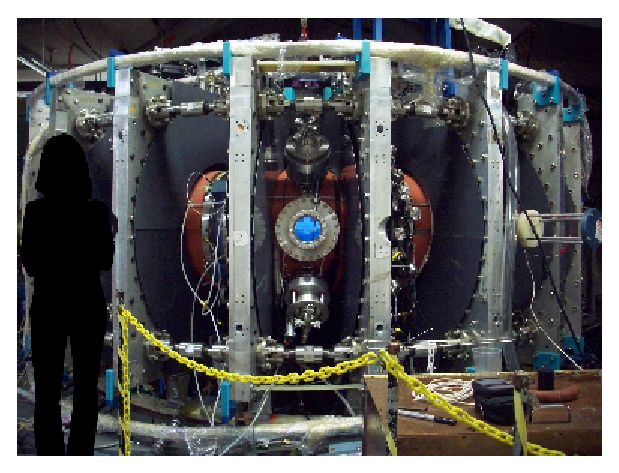
\includegraphics[width=0.8\hsize]{eps/tokamak.eps}
 \caption{The HBT-EP ``Tokamak'' at Columbia University.}
 \label{fig:tokamak}
\end{figure}

Plasma control for fusion is an applications of energy CPS, where
complex algorithms must be computed at a very high rate.
Figure~\ref{fig:tokamak} shows the HBT-EP Tokamak at Columbia
University~\cite{Maurer_PPCF11,Rath_FED12} that magnetically controls
the 3-D perturbed equilibrium state of the plasma~\cite{Boozer_PP99}.
It is required to process 96 inputs and 64 outputs of 16-bit data at a
sampling rate of a few microseconds.
An initial attempt of the Columbia team employed fast CPUs or FPGAs, but
even the simplified algorithm failed to run within 20$\mu$s.
An alternative approach was to parallelize the algorithm using the
graphics processing unit (GPU) and CUDA~\cite{CUDA} -- the most
successful massively parallel computing technology.
However, the current system for GPU computing is not designed to
integrate sensor and actuator devices with the GPU.
This is attributed to the fact that the current software stack
of GPU computing is independent of I/O device drivers.
Since it might take tens of microseconds to transfer hundreds-of-bytes
data between the CPU and the GPU, it is not affordable for the current
software stack to apply the GPU for plasma control in real-time.
This is a signficant problem not only for plasma control but also for
any applications of CPS that are augmented with compute devices.

In order to utilize the GPU for applications of CPS, the system is
required to support a method of bypassing data transfer between the GPU
and the CPU, instead connecting the GPU and I/O devices directly.
To the best of our knowledge, however, there is currently no generic
systems support for such a direct data transfer machanism except for
specialized commercial products for the InfiniBand
network~\cite{GPUDirect}.
As a way of eliminating the data transfer cost between the CPU and the
GPU, the current programming framework often supports host memory
allocation, which enables the GPU to access data on the host memory;
however, it is unclear if this scheme is best suited for low-latency GPU
computing, because the data access to the host memory from the GPU is
expensive.
Given that GPUs are increasingly deployed in the domain of
CPS~\cite{Hirabayashi_REACTION12, Mangharam11, McNaughton_ICRA11,
Michel_IROS07}, 
and basic real-time resource management techniques for the GPU started to be
disclosed \cite{Elliott_RTS12, Elliott_ECRTS12, Kato_RTAS11,
Kato_RTSS11, Kato_ATC11, Kato_ATC12, Liu_PACT12}, it is time to look
into a tight integration of I/O processing and GPU computing.

\textbf{Contribution:}
In this paper, we present a zero-copy I/O processing scheme for GPU
computing.
This scheme enables I/O devices to directly transfer a limited size of
data to and from the GPU, by coordinating their device drivers. 
We also investigate a possibility of the exisiting schemes to support
low-latency GPU computing, and identify an advantage of our new scheme.
To do so, we provide a case study using the Columbia University's
Tokamak plasma control system that demonstrates an effect of our
new scheme on a sampling period of plasma control.
Furthermore, we provide microbenchmarking results to evaluate more
generic properties of the I/O processing schemes
By clarifying these capabilities, we aim to not only improve the overall
performance but also broaden the scope of CPS that can benefit from the
state-of-the-art GPU computing technology.

\textbf{Organization:}
The rest of this paper is organized as follows.
Section~\ref{sec:system_model} describes the system model and
assumptions behind this paper.
Section~\ref{sec:io_processing} presents our zero-copy I/O processing
scheme, and differentiates it from the exisiting schemes.
\section{Case Study}
\label{sec:case_study}

In this section, we provide a case study of magnetic control of
perturbed plasma equilibria using the HBT-EP ``Tokamak'' equipped with
the GPU and the presented I/O processing schemes.
This control system requires low latency and high computing capabilities
to achieve a sampling period of the order of ten microseconds, while
processing 96 inputs and 64 outputs of 16-bit data with a complex
algorithm.
As mentioned in Section~\ref{sec:introduction}, the CPU implementation
of this algorithm has never met the requirement of computing power.
The case study presented herein, therefore, is significant in that we look
into a possibility of GPU implementations for the plasma control system.

\begin{figure}[t]
 \centering
 \includegraphics[width=\hsize]{eps/tokamak_sysarch.eps}
 \caption{HBT-EP magnetic sensors and control coils connected with the
 GPU.}
 \label{fig:tokamak_sysarch}
\end{figure}

Figure~\ref{fig:tokamak_sysarch} shows a system architecture used in
this case study.
The control input comes from a set of magnetic sensors through a D-TACQ
ACQ196 digitizer, and the resulting control signal is sent to two D-TACQ
AO32 analog output modules to excite control coils.
These input and output modules are connected to the GPU upon the PCIe
bus.
We evaluate three different schemes against this system architecture
from the viewpoint of the cycle time of algorithm execution and the
latency of data transfer. 
Each scheme is applied as follows:
\begin{itemize}
 \item In the {\hd} scheme, the device driver of the digitizer transfers
       the input data set to the buffers allocated on the host memory.
       The control program copies this data set to the device memory via
       PCI-mapped host memory space, and the parallelized control
       algorithm runs on the GPU with the data on the device memory.
       Once the output data set is produced by the GPU, the control
       program copies it back to the host memory, and it is finally
       pulled by the device driver of the analog output modules.
       This is the traditional form of GPU computing.
 \item The {\hp} scheme pins the input and output buffers to PCI-mapped
       host memory space.
       Since the data set pushed and pulled by the device drivers of
       the I/O modules is directly accessible to the GPU, there is no
       need to perform data copies.
       However, this scheme must compromise the latency of data access
       imposed on the GPU when executing the control algorithm.
 \item Similarly to the {\hp} scheme, the {\dm} scheme proposed in this
       paper uses pinned PCI-mapped host memory space to allocate the
       input and out buffers, and further maps it to the device memory
       through PCI BAR space.
       Thus, there is no need of data copies while the data access of
       the control algorithm is limited within the device memory.
\end{itemize}

\begin{figure}[t]
 \centering
 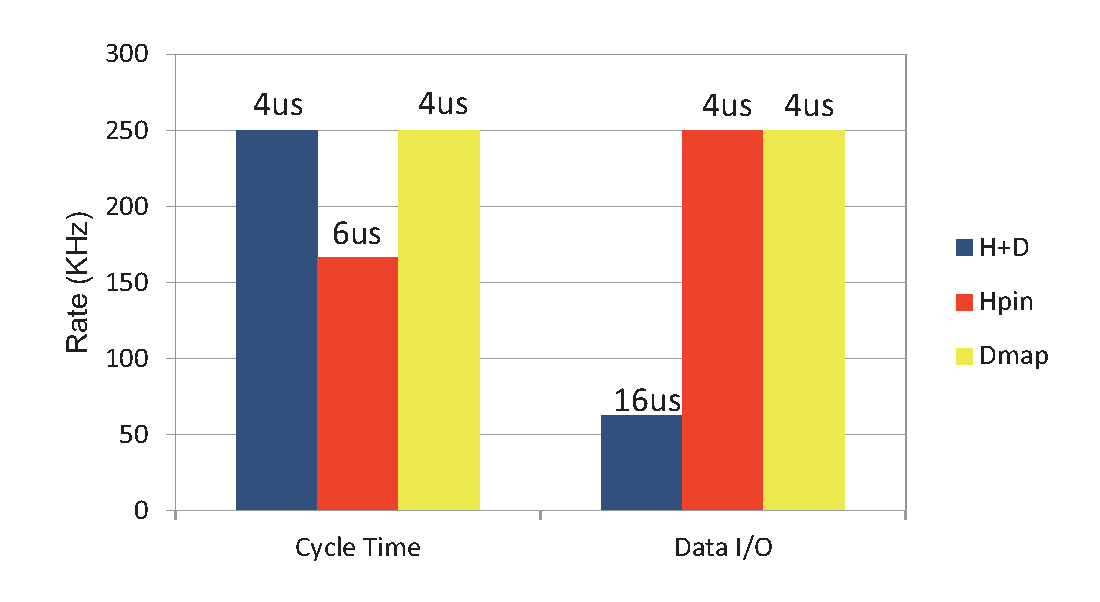
\includegraphics[width=\hsize]{eps/eval_plasma.eps}
 \caption{Cycle time and latency of the plasma control system.}
 \label{fig:eval_plasma}
\end{figure}

We now demonstrate that our zero-copy I/O processing scheme reduces both
the cycle time of algorithm execution and the latency of data transfer
in this control system.
Figure~\ref{fig:eval_plasma} shows the result of experiments conducted
under the three different schemes, respectively.
Apparently, the {\dm} scheme achieves the highest rate in both algorithm
execution and data transfer.
The remaining two schemes, on the other hand, compromise either of them.
It is fairly reasonable to observe that the {\hd} and the {\dm} schemes
exhibit the same performance level for algorithm execution since they
both use the device memory, while the latency of data transfer is
equivalent between the {\hp} and the {\dm} schemes since they both
remove data copies.
Comparing the {\hd} and the {\hp} schemes, one can also observe that the
impact of overhead introduced by data copies, \textit{i.e.}, $16\mu$s, is
greater than that introduced by the GPU accessing pinned host memory
space, \textit{i.e.}, $6\mu$s, on the overall system performance.
Curiously, there is additional latency of $4\mu$s observed when running
the control system.
We suspect that this latency comes from some interactions among the host
computer, the graphics card, and the I/O modules.
Lessons learned from this evaluation are summarized as follows:
\begin{itemize}
 \item Zero-copy I/O processing is very effective for this control
       system, reducing the latency of data transfer from $16\mu$s to
       $4\mu$s.
       The speed-up ratio is 4$\times$.
 \item Furthermore, the {\dm} scheme proposed in this paper reduces the
       cycle time of algorithm execution from $6\mu$s to $4\mu$s.
       The speed-up ratio is 1.5$\times$.
       Since the HBT-EP ``Tokamak'' accommodates up to 216 inputs,
       meaning that the cycle time of algorithm execution is more
       dominated by data accesses, the benefit of the {\dm} scheme over
       the {\hp} scheme would be more significant for a larger scale of
       plasma control.
\end{itemize}

\begin{figure}[t]
 \centering
 \includegraphics[width=0.85\hsize]{eps/oscilloscope.eps}
 \caption{Screenshot of the oscilloscope.}
 \label{fig:oscilloscope}
\end{figure}

The above measurement explains that the control system can operate at a
sampling period of $16\mu$s.
The data transfer from and to the input and output modules takes $4\mu$s
each.
The algorithm execution takes $4\mu$s.
Adding additional latency of $4\mu$s, the total control rate must be
able to achieve $16\mu$s.
Figure~\ref{fig:oscilloscope} depicts the screenshot of the oscilloscope
where we measure the signals of the input and the output modules.
The topmost and middle signals represent the input and the output,
respectively, while the lower signal indicates the base clock.
The grid spacing of the X axis is $5\mu$s.
The time interval from the first downward edge in the clock signal after
the input signal goes up to the instant when the output signal starts
uprising is almost equal to $16\mu$s.
This means that the total control processing time is $16\mu$s. 

We next demonstrate that the control system is running properly at a
rate of $16\mu$s.
The control input comes from a set of magnetic sensors arranged in a
ring, as illustrated in Figure~\ref{fig:tokamak_sysarch}, and the
magnetic field that they measure is rotating, whose orientation is
described by a \textit{phase}.
Ideally, the phase is equivalent to multiplication of time and
frequency.
To control this mode, the control system needs to produce a control
signal that generates an equal and opposite field, which also needs to
rotate.
Obviously, the two fields should have a constant phase difference,
because it is given by multiplication of the control processing time and
the rotation frequency.
However, in practice, the rotation frequency is not constant but is
changing.
As a result, the phase difference appears to oscillate, with the base
output signal, which can be found as spikes in
Figure~\ref{fig:phase_base}.
Now, we measure the phase difference with the output signal time-shifted
by $16\mu$s.
In other words, the effective control system latency is reduced by
$16\mu$s.
As shown in Figure~\ref{fig:phase_shifted}, the spikes are now all
removed.
This indicates that the control system is perfectly in phase with the
mode, and the effective control system latency now must be zero,
\textit{i.e.}, the actual latency is $16\mu$s.

\begin{figure}[t]
 \centering
 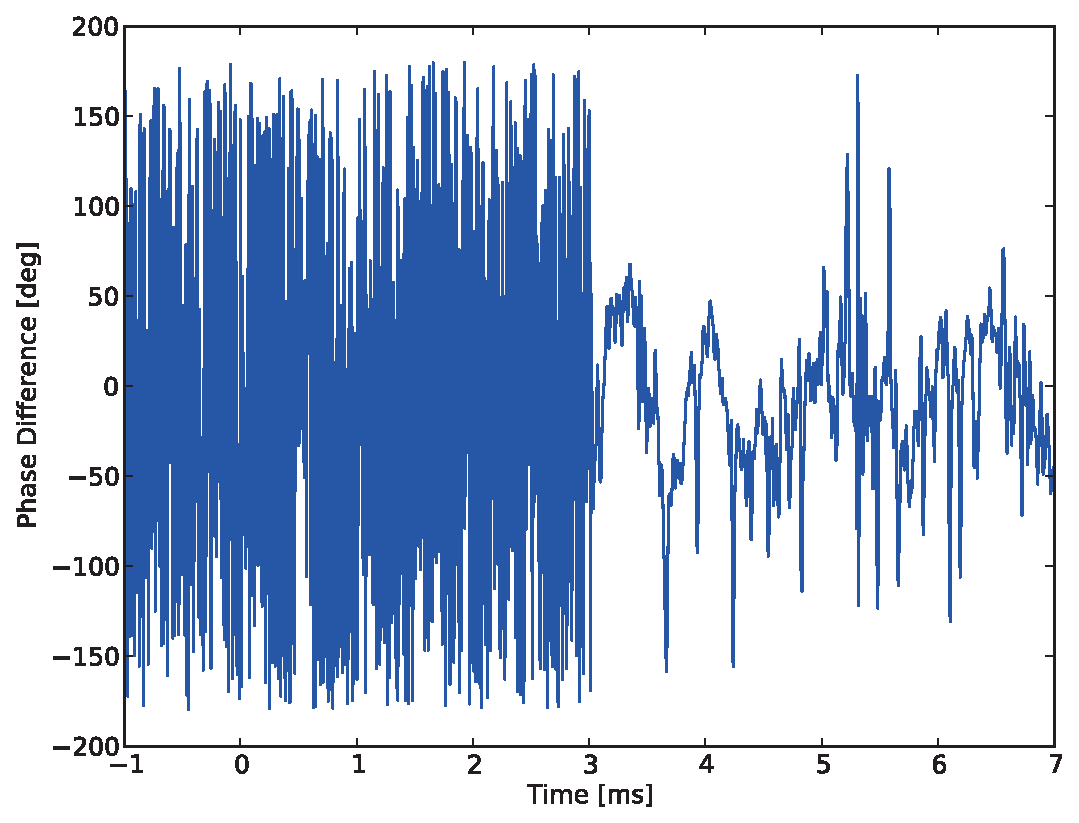
\includegraphics[width=0.7\hsize]{eps/75221_base.eps}
 \caption{Phase difference observed with the base output signal.}
 \label{fig:phase_base}
\end{figure}
\begin{figure}[t]
 \centering
 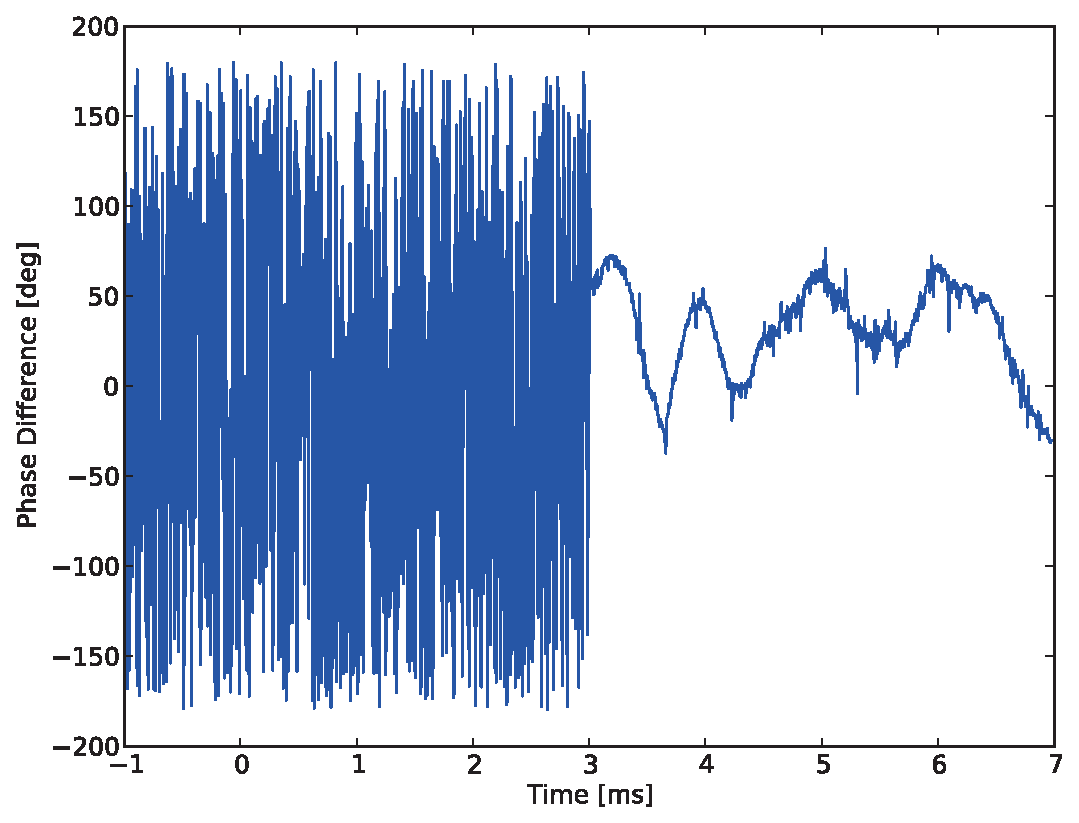
\includegraphics[width=0.7\hsize]{eps/75221_shifted.eps}
 \caption{Phase difference observed with the output signal shifted by 16$\mu$s.}
 \label{fig:phase_shifted}
\end{figure}

\begin{figure}[t]
 \centering
 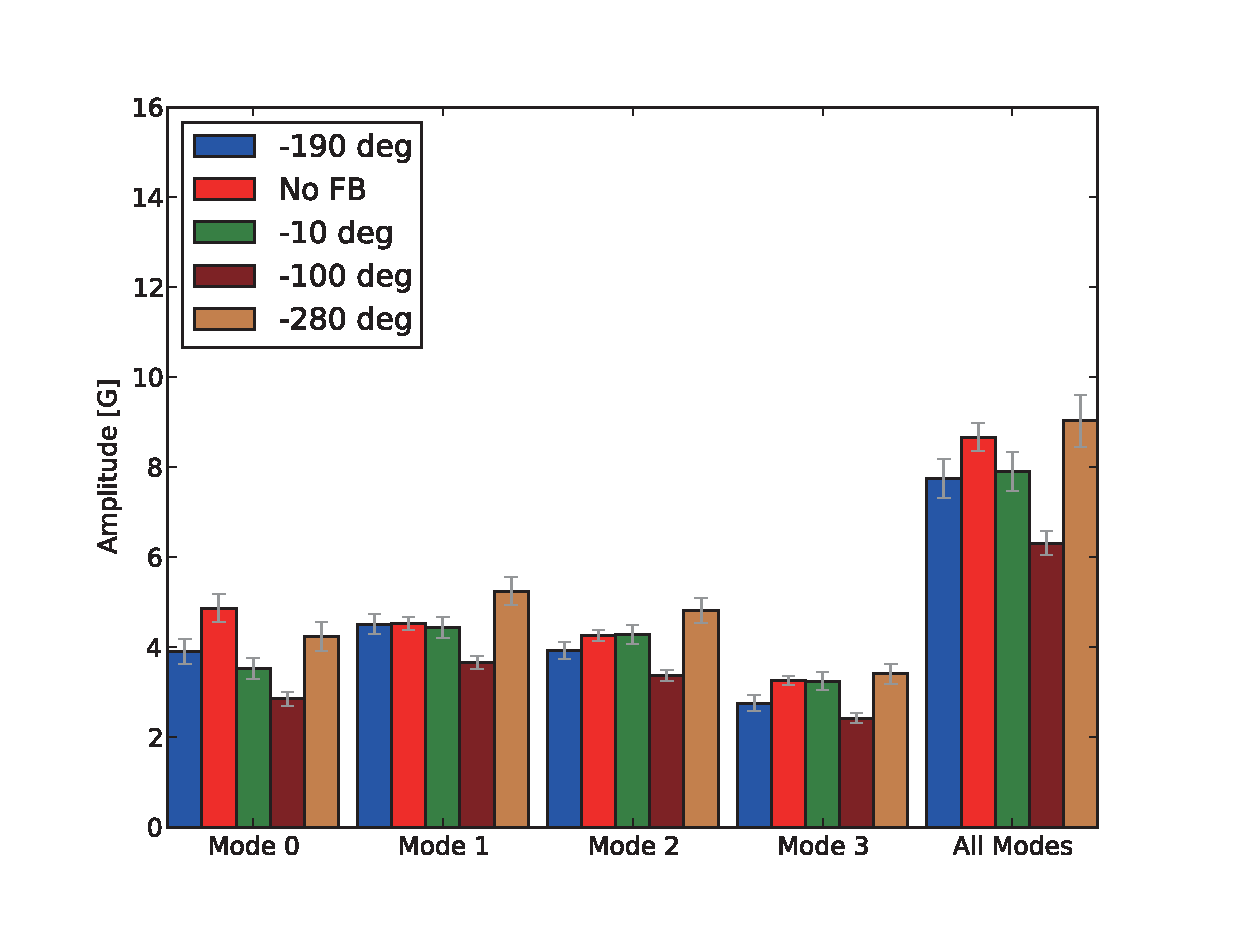
\includegraphics[width=0.9\hsize]{eps/overview.eps}
 \caption{Practical findings of plasma control.}
 \label{fig:plasma_overview}
\end{figure}

Finally, we discuss practical findings of plasma control regarding the
HBT-EP ``Tokamak'' device.
Figure~\ref{fig:plasma_overview} shows a comparison of the average
perturbation amplitudes with different phasings.
The control system incorporates four arrays of magnetic sensors and
control coils, each of which controls one specific mode.
They are placed at different poloidal angles around the toroidal ring.
Due to their different locations, they measure slightly different
amplitudes.
From this experiment, we find that feedback at 280 degrees excites
perturbation, while feedback at 100 degrees is the right range for
suppression.
As compared to no feedback scenario (``No FB'' in the figure), for
example, we find that we can supress the strength of the rotating field
by up to 30\% for any mode observed in this experiment.
\section{Benchmarking}
\label{sec:benchmarking}

To evaluate our system we compared it with the vendor provided methods
mentioned in section \ref{sec:data_communication}. Timing analysis of
addition and multiplication of varying sized matrices was performed
(two common benchmarks also used in related work
\cite{Rossbach_SOSP11}). Since our focus is on data access and
communication (not computation) we chose matrix addition as a benchmark as it is a
straightforward operation for a GPU to perform. Matrix multiplication
is also included to briefly illustrate how increasing computational
complexity and data accesses affect time to completion. Effective host read and write throughput for each method was also analyzed.

\subsection{Matrix Operations}
Figure \ref{fig:madd_time_spent} shows where the system spends its time in performing a 2048x2048 integer matrix addition using each of the four methods. The time categories are as follows:

\begin{itemize}
 \item {\bf Init: }GPU initialization time.
 \item {\bf MemAlloc: }Memory allocation time (host and/or GPU).
 \item {\bf DataInit: }Time to initialize the matrices.
 \item {\bf HtoD: }Copy time from host to device (\hd).
 \item {\bf Exec: }Execution time of the kernel function.
 \item {\bf DtoH: }Copy time from device to host (\hd\ and \dmh).
 \item {\bf DataRead: }Time to read the result.
 \item {\bf Close: }Free memory and close GPU.
\end{itemize}

\begin{figure}[tb]
\centering
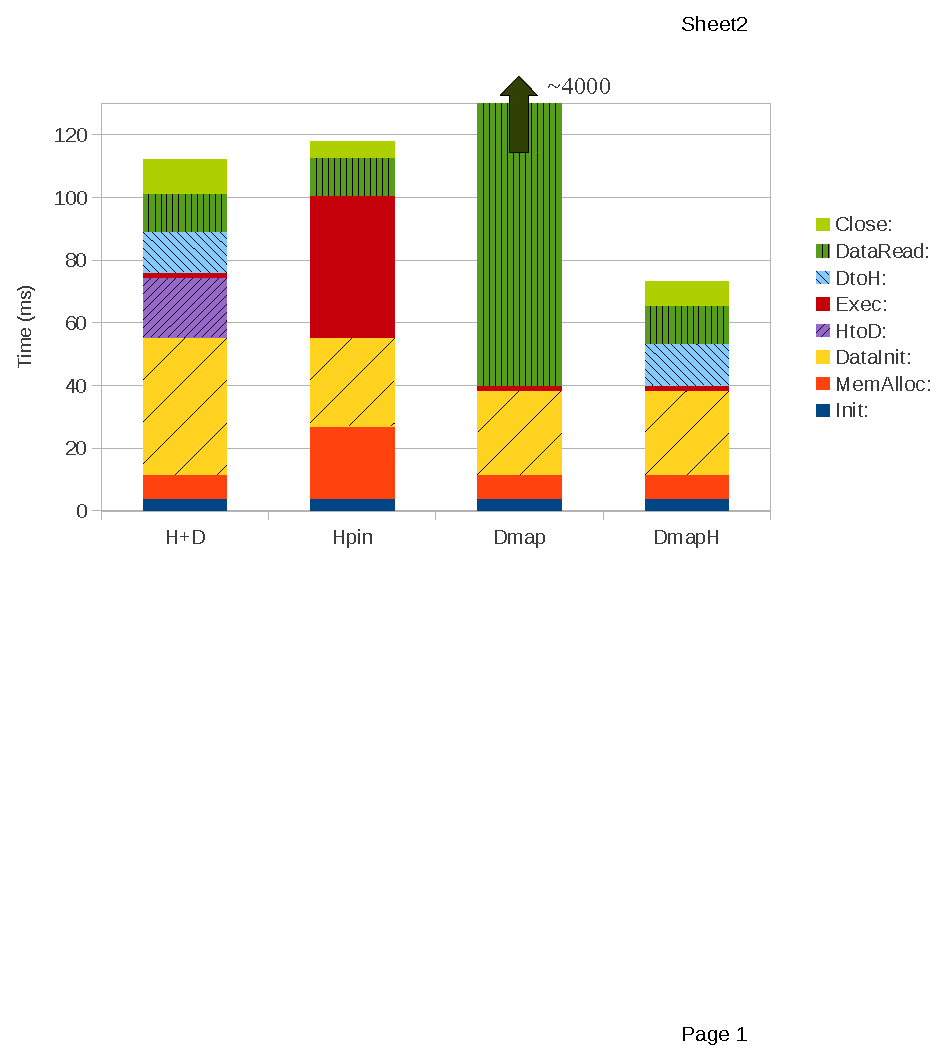
\includegraphics[width=0.5\textwidth, trim=0.0in 3.25in 0.0in 0.25in, clip=true]{eps/madd_time_spent.eps}
\caption{Matrix addition}
\label{fig:madd_time_spent}
\end{figure}
\begin{figure}[tb]
\centering
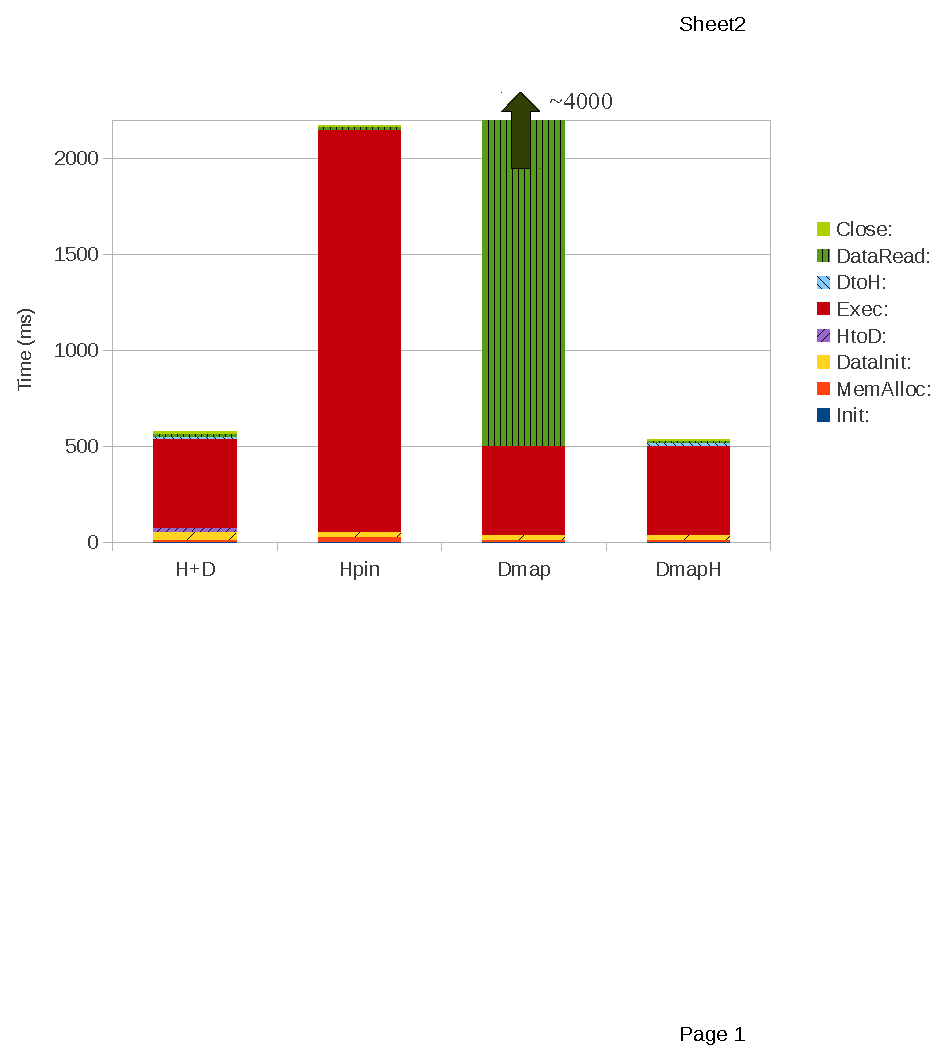
\includegraphics[width=0.5\textwidth, trim=0.0in 3.0in 0.0in 0.5in, clip=true]{eps/mmul_time_spent.eps}
\caption{Matrix multiplication}
\label{fig:mmul_time_spent}
\end{figure}

First, looking at figure \ref{fig:madd_time_spent} it is clear that using our
\dmh\ method the total time to completion is less than the
others ($34\%$ less than its nearest competitor, \hd). More interesting is the
comparison of how much time is spent for each sub-task. 

For most time categories \dmh\ seems to enjoy the best of each of the
other three: The memory allocation time for \dmh\ is nearly identical to that of
\hd\ and \dm\ and clearly less than \hp. The same is true for the
execution times. Similarly, for data initialization, \dmh\ is just as good
as \hp\ and \dm\ which are superior to \hd. 

\begin{figure}[tb]
\centering
\includegraphics[width=0.45\textwidth, trim=0.0in 2.0in -0.3in 0.74in, clip=true]{eps/madd_time.eps}
\caption{Total Matrix Addition Times}
\label{fig:madd_time}
\end{figure}
\begin{figure}[tb]
\centering
\includegraphics[width=0.45\textwidth, trim=0.0in 2.0in -0.3in 0.72in, clip=true]{eps/mmul_time.eps}
\caption{Total Matrix Multiplication Times}
\label{fig:mmul_time}
\end{figure}

\begin{figure}[t]
\centering
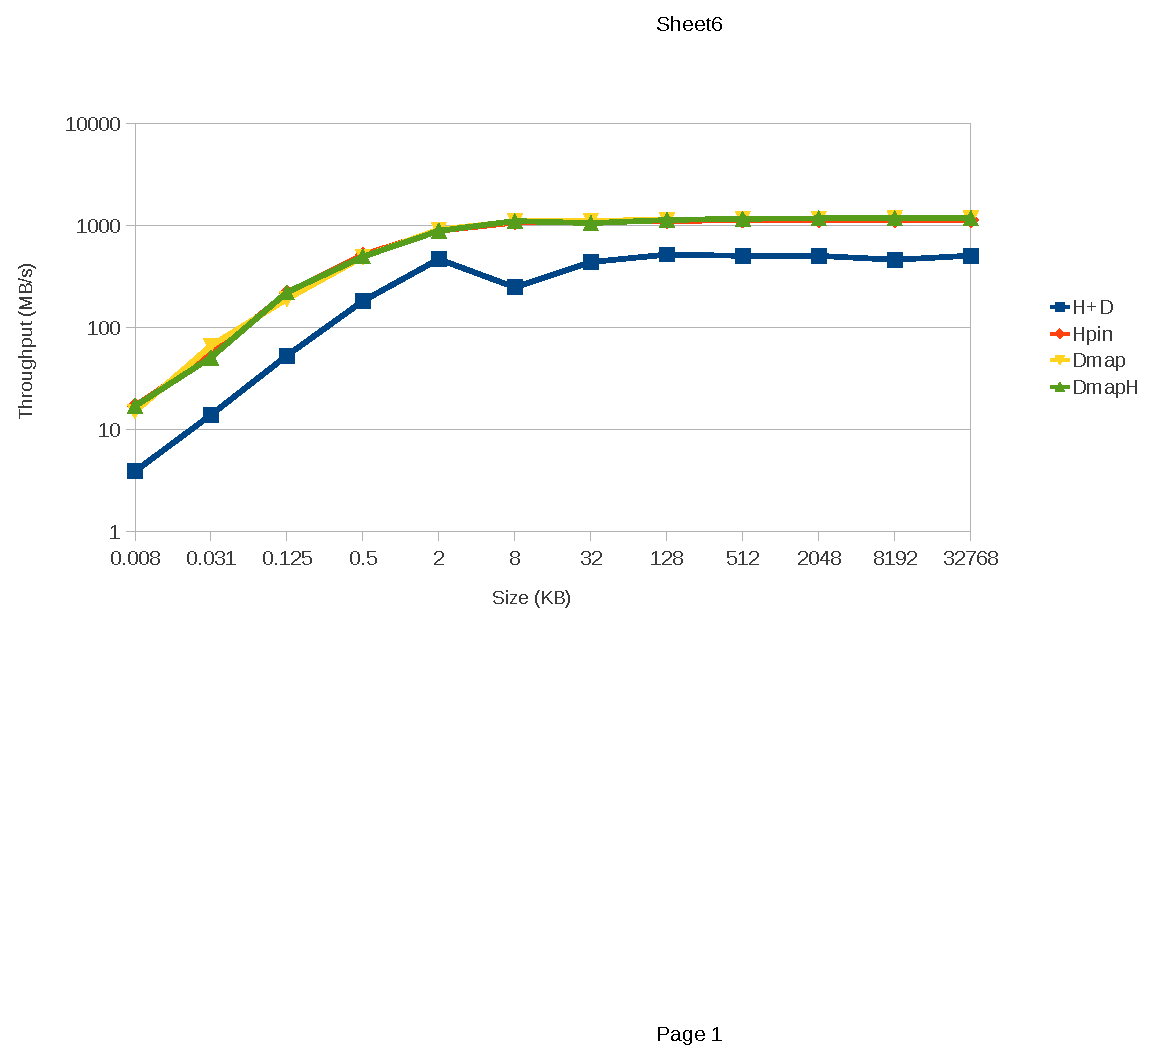
\includegraphics[width=0.45\textwidth, trim=0.0in 2.75in -0.1in 0.60in, clip=true]{eps/write_tput.eps}
\caption{Host Write Throughput}
\label{fig:write_tput}
\end{figure}
\begin{figure}[tb]
\centering
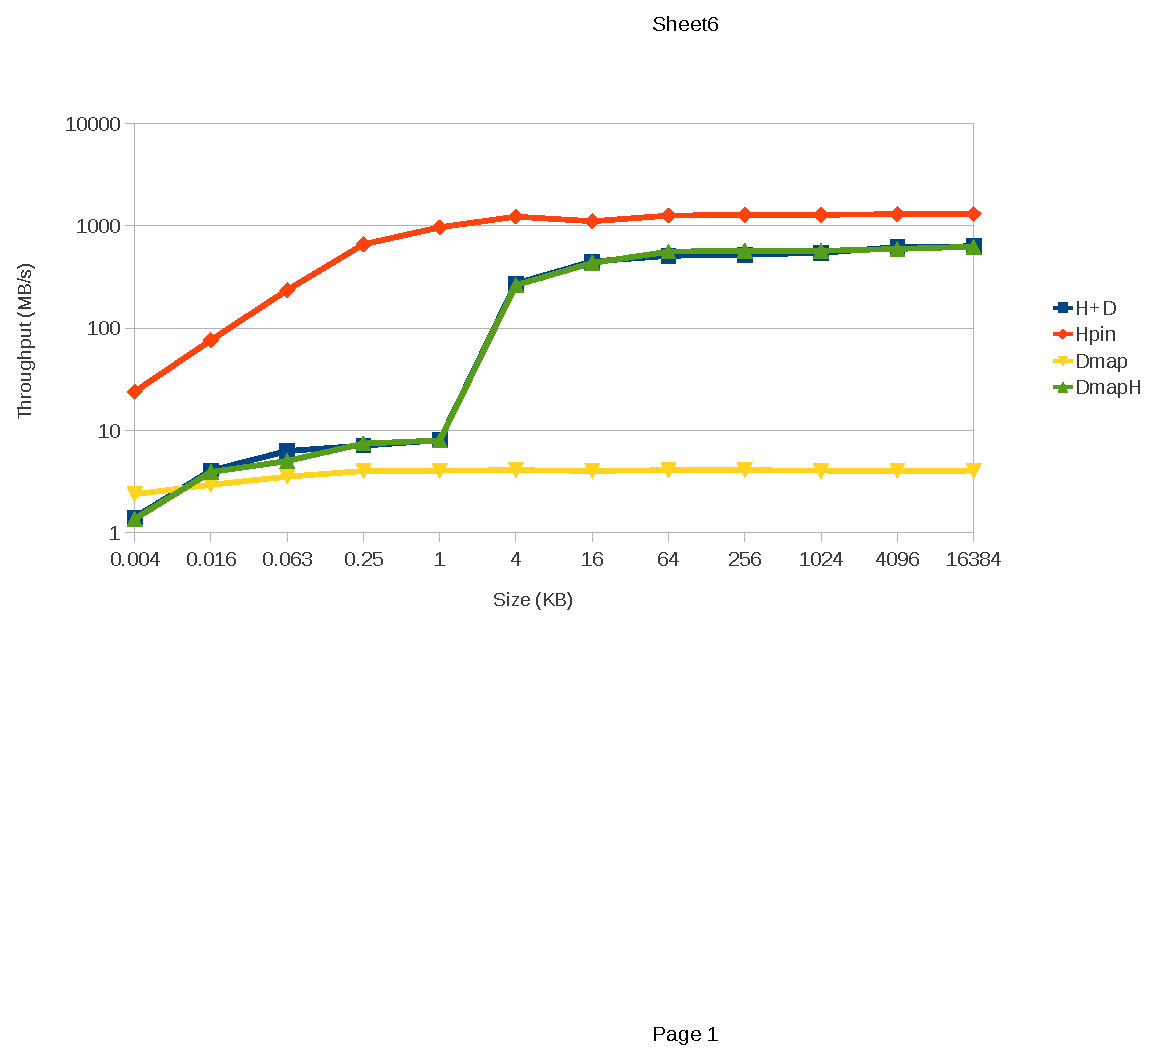
\includegraphics[width=0.45\textwidth, trim=0.0in 2.5in -0.1in 0.6in, clip=true]{eps/read_tput.eps}
\caption{Host Read Throughput}
\label{fig:read_tput}
\end{figure}

The most notable difference among the four methods is the data read time for \dm\ which is orders of magnitude greater than the rest. This represents 16MB of data, read 4 bytes at a time across the system buses and is the motivation for our \dmh\ method. Instead of reading one matrix element at a time, \dmh\ first copies the data to the host before reading.

The same anomaly is present in the execution time for \hp\ -- the GPU must read one element at a time from the host memory (in the other three methods the data reside on the GPU during computation). This makes \hp\ increasingly inferior as data sizes grow.

Figure \ref{fig:mmul_time_spent} shows the same time analysis for matrix multiplication. The only difference occurs in the execution times. This is not surprising as the multiplication experiments are exactly the same as addition with the exception of the kernel function on the GPU. In fact, if execution times were omitted, figures \ref{fig:madd_time_spent} and \ref{fig:mmul_time_spent} would look identical.

%One thing to note, however, is the amount by which the execution times have increased. For each element in the output matrix, there will be $2n$ data reads, $n$ multiplications, and $1$ data write where $n$ is the length and width of the matrices (as opposed to $2$ accesses, $1$ addition and $1$ write).   

While this does present a real-world scenario, in a real-time system it is
more likely that tasks will be performed repeatedly and therefore
the GPU initialization and closing costs might occur only once -- the
same context with kernel function(s) loaded would remain active while
only the data might change. Furthermore, it could be the case that the
memory allocated for the task could be reused and only the contents
modified. For these reasons, the remainder of our analysis focuses only on reads, writes, transfers, and execution. 

Figure \ref{fig:madd_time} shows the time to completion of matrix
addition as a function of matrix size (note the logarithmic
scale). \hp\ appears to be the best performer until a matrix size of
$32\times32$ (corresponding to a data size of 4KB for each matrix) at
which point \dmh\ becomes superior. This is also reflected in the
matrix multiplication times (figure \ref{fig:mmul_time}). One thing to
note is the growth rate of \hp\ in matrix multiplication; Since each
thread must perform multiplication and addition $n^2$ times (compared
with one addition in matrix addition), the number of reads that occur
across the buses increases by a greater exponential factor. We expect that the time for \hp\ would eventually surpass \dm\ as the trend in the graph indicates.


%Note that even with the logarithmic time scale the curves appear exponential because while the matrix length and width increase as $2^n$ the data size of the
%matrix is $2^n \times 2^n \times 4 =  2^{2n+2}$ bytes (for 32-bit integers).


\subsection{Data Throughput}
Figure \ref{fig:write_tput} shows the effective host write throughput
as a function of data size.  We use the term `effective throughput' to
mean ($size/time$) where $time$ is measured from the beginning of data
initialization to the point at which it is actually available to
the GPU. For example, in the case of \hd\, this corresponds to the total time for the host to write to each element in the data structure (which
is in main memory) plus the time to copy the data to the GPU.

Figure \ref{fig:write_tput} shows that the write throughput of \dmh\
is better than \hd\ by about a factor of 2 and at least as good as the others (\hp, \dm, and \dmh\ all coincide
almost exactly in the graph). Figure \ref{fig:read_tput} paints a
slightly different picture for read throughput. It should not be
surprising that \hp\ outperforms the rest as it represents the host
iterating over a data structure that is already in host memory. \hd\
and \dmh, on the other hand, must first copy the data from the GPU to
the host and they achieve roughly equal performance (they coincide in
the graph). Finally, \dm\ is
the weakest performer because of the large number of small reads that
occur across system buses (as explained earlier).


\bibliographystyle{abbrv}
\bibliography{references}

\end{document}
